%===================================== CHAP 4 =================================

\chapter{Neural Linear Bayesian Regression Model}\label{ch:bdqn}

A major drawback of the methods discussed in chapter \ref{ch:linear} is that they are all linear models. These cannot perform well in environments with complex non-linear relationships between state-action pairs and Q-values without significant feature engineering. Recent developments in the RL field focus on deep RL\citep{mnih_2015, mnih_2016,silver_2017} where neural networks are used as encode these relationships allowing succesfull results on complex games. As such it it would be beneficial to be able to combine the methods from chapter \ref{ch:linear} with more complex models. This chapter attempts this and tests the new model on multiple complex environments with comparisons to other popular deep RL methods.

\section{Combining Bayesian Q-learning with Neural Networks}

\subsection{Neural Linear Model}

Without significant feature engineering a linear model cannot generalize to more complex non-linear relationships between state-action pairs and their Q-values. However using bayesian methods with non-linear models can be difficult and computationally heavy. \cite{carlos_2018} compared a large array of bayesian models on a set of bandit environments. They found that accurate complex models often performed worse than simpler approximate methods. The suggested reason for this is that complex models require more data and training to acheive reasonable variance estimates. Since RL is an online task this can lead to miscalibrated variance early on in the training process that leads to worse results.

Emperically \cite{carlos_2018} finds what they coin as a neural linear model to work best. The model consists of using a neural network as a basis function that is used as the covariates to a linear bayesian regression model. This is equivalent to rewriting the regression task to 

\begin{equation*}
	Q = \phi(X)\beta + \varepsilon \quad \text{where} \quad \varepsilon \sim N(0,\sigma^2)
\end{equation*}

where $\phi(X)$ is the neural networks output given an input $X$. The error in the bayesian regressions point estimates is backpropagated through the neural network to learn a useful basis function. Note that this means the bayesian regression no longer incorporates all the uncertainty since the above assumes no uncertainty in the $\phi(X)$ encoding. \cite{carlos_2018} suggests that error that comes with this assumption is counteracted by the models stable uncerainty estimates.

This setup allows the application of the methods discussed in chapter \ref{ch:linear} in more complex environments. It is also this method \cite{azziz_2018} follows in their application of the BN model to more complex models.

\subsection{Bayesian DQN Models}

Based on the results of \cite{carlos_2018} this thesis attempts to combine neural networks and the BNIG model through a neural linear setup. To start off a summary of the archicture used in \cite{azziz_2018}, called the BDQN, is provided. This is used as a base which will modified to fit with the BNIG model and thus allow for better variance propagation.

\subsubsection{BDQN Model}

The BDQN architecture starts with the same archicture as the standard DQN architecture\citep{mnih_2015}. The final layer of a DQN is a linear layer which means it can be replaced by any linear model. \cite{azziz_2018} replaces this with a BN model. This model is trained using the posterior updates described in chapter \ref{ch:linear} in equation \ref{eq:known_noise_posterior_update}. The neural network is trained using the loss function

\begin{equation*}
	\theta = \theta - \alpha\nabla_\theta\big(Q_t - [\mu_n^T\phi_\theta(x_t)]\big)^2.
\end{equation*}

The only difference to a regular neural network is that the networks output estimate is replaced by the MAP estimate of $\beta$. One could replace the MAP estimate by samples from the posterior $Q$. However as shown in the linear case this should have no effect on the final estimate but does have a higher computational cost than simply using that MAP estimate.

These two training processes do not have to happen sequentially. In \cite{azziz_2018} the neural network is updated as frequently as in the original DQN implementation, while the bayesian regression trained from scratch every 10,000 steps on either 100,000 datapoints or the entire replay buffer if it contains less. This is done to handle the non-stationarity of the task. 

\subsubsection{Modification to a BNIG DQN model}

The downside retraining the bayesian regression is that this is computational heavy, especially considering that the final layer in the neural network consists of 512 neurons, meaning the update requires matrix arithmetic with a 512 by 512 matrix. On top of this using a BNIG model requires the target Q-values to be sampled from the posterior. This means every 10,000 steps 100,000 samples must be calculated which requires matrix arithmetic of the same magnitude. Instead this thesis considers the exponential forgetting method. However implementing this requires some extra considerations to ensure that the model remains stable.

Recall that the classic DQN has one online network that is updated each training step and one target network that is updated occaisonally to match the online network. \cite{mnih_2013} found that using this target network to calculate the regression target helped stabalize the algorithm.

With exponential forgetting the bayesian regression is trained continuosly. However, using the online bayesian regression method to calculate targets based on the output from the target network will lead to instability. The regression model can train on thosands of datapoints from the online network between network syncs. Using different network encodings with the same bayesian regression will lead to different results which will increases the loss. An increased loss leads to larger network changes which amplifies the effect leading to instability.

To deal with this issue the same setup that is used for the networks is used for the regression models. Two bayesian regression models are created, one online and one target. The target model is used to calculate the target action-values while the online model is used for decision making. The target model is then updated to the parameters of the online model when the target network is updated. This decreases the loss and resulted in a stable network.

With this approach the only required change to transform this to a BNIG setup is to swap out the bayesian model used in the BDQN with the BNIG model and sample action-values from the posterior for both the online and target models.

\section{BNIG DQN Implementation}

\todo Pseudocode, Architecture

\section{BNIG DQN Results}

In this section the BNIG DQN is tested on a variety of environments and compared to a regular DQN. 

To ensure a correct implementation of the DQN and a fair comparison to the BNIG DQN the python package Dopamine\citep{castro_18} was used. This package contains an implementation of a DQN that matches the baselines of the \cite{mnih_2015}. The BNIG DQN was implemented ontop of this DQN implementation.

The Dopamine package has hyperparmeters for the DQN on many of the tested environments. These are used for both the DQN and BNIG DQN in the following tests. A table of the hyperparmeters per environment is provided in the appendix.

The comparison of the two methods is based on their performance on the environment relative to the number of samples it has trained on. To fairly compare the methods during training the experiments the results are gathered from an evaluation stage. The evaluation stage is run every time one wants to measure the performance of the method and consists of calculating the average total reward over a few episodes.

In this evaluation phase the model and network are not trained. The DQN agent acts greedily without any probability of doing an action. The BNIG DQN acts greedily with respect to it's MAP estimate. This means it acts based on the mean $\beta$ values and no noise.

\subsection{Corridor}

\todo

\subsection{Cartpole}

The environment considered is a classic toy example called cartpole. The environment was first proposed in \cite{barto_sutton_1983} and is easily available through the Open AI gym environment \citep{brockman_2016}.
\todo figure to illustrate 
The task consists of balancing a pole on top of a cart. If the pole falls over 15 degrees from the upright position or if the cart goes too far (2.4 units from the center) to the left or right the game is terminated. The game is also terminated after 500 timesteps. Every timestep a reward of $+1$ is received. There are two actions, the cart can be pushed to the left or to the right at every timestep. There are 4 input variables that define the state: the pole angle from vertical, the position of the cart and the derivative of both variables. 

The environment implementation from OpenAI Gym was used \citep{OpenAI_gym}. Each method was run for 50,000 steps with 10 different seeds and every 1000 steps an evaluation phase is run over 1000 steps. The results are summarized in \ref{fig:nn_cartpole}

\begin{figure}[H]
    \centering
    \subfloat[DQN]{
        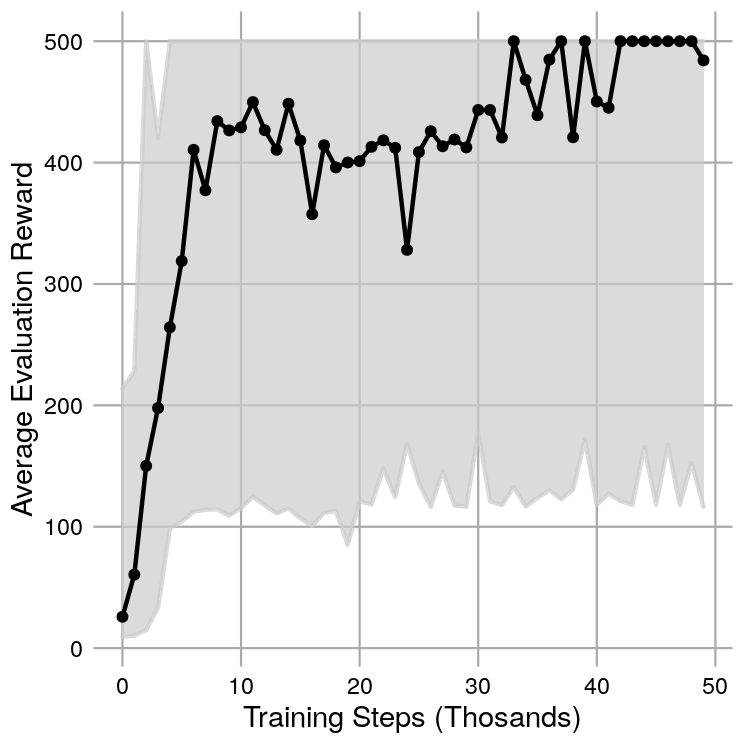
\includegraphics[scale=0.5]{DQNCartpole.png}
    }
    \subfloat[BNIG DQN]{
        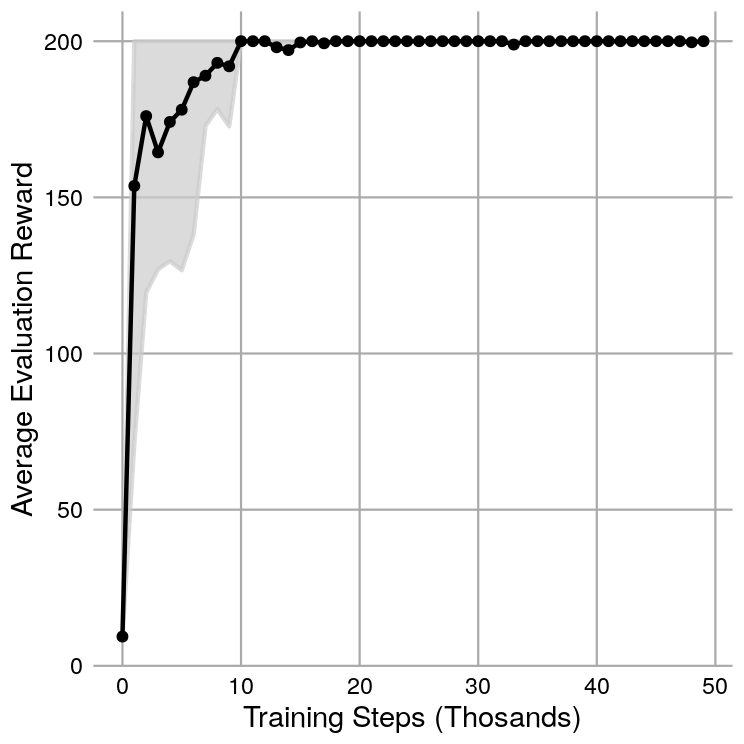
\includegraphics[scale=0.5]{BDQNCartpole.png}
    }
    \caption{\textbf{DQN and BNIG DQN Performance on Cartpole}: Plots show the mean performance over 10 different attempts. The shaded area covers 80\% of the total reward over all attempts.}
    \label{fig:nn_cartpole}
\end{figure}

\subsection{Acrobot}

Another common toy example is called acrobot. The experiment is first described in \cite{hauser_1990} and put into an RL context in \cite{sutton_1996}. The environment consists of a robot arm with two joints, one fixed to the origin and one with an actuator. The arm starts hanging downwards under the origin. The goal is to get the end of the robot arm over a line above the origin which terminates the episode. A reward of $-1$ is given each timestep. There are three actions, apply 1 torque left, 1 torque right or no operation. The state input is

$$
[\cos(\theta_1), \sin(\theta_1), \cos(\theta_2), \sin(\theta_2), \dot{\theta}_1, \dot{\theta}_2]
$$

where $\theta_1$ is the angle of the first joint and $\theta_2$ is the angle of the second joint relative to the first.

\todo figure to illustrate 

The environment implementation from OpenAI Gym was used \citep{OpenAI_gym}. Each method was run for 50,000 steps with 10 different seeds and every 1000 steps an evaluation phase is run over 1000 steps. The results are summarized in \ref{fig:nn_acrobot}


\begin{figure}[H]
    \centering
    \subfloat[DQN]{
        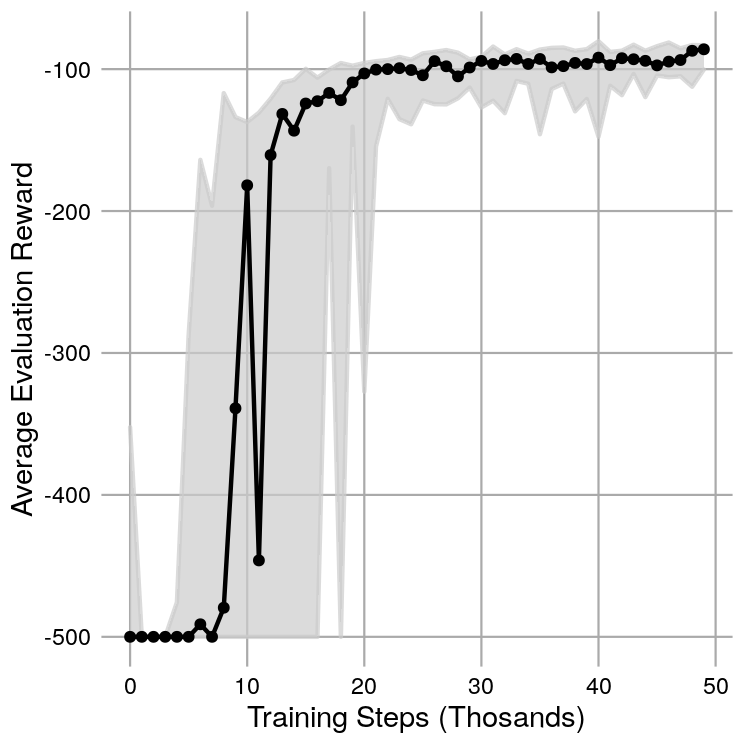
\includegraphics[scale=0.5]{DQNAcrobot.png}
    }
    \subfloat[BNIG DQN]{
        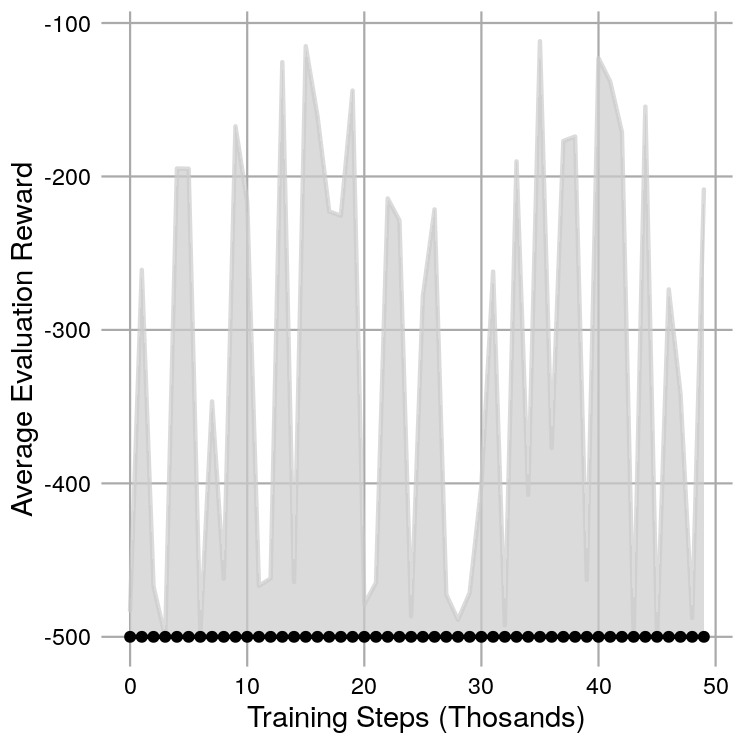
\includegraphics[scale=0.5]{BDQNAcrobot.png}
    }
    \caption{\textbf{DQN and BNIG DQN Performance on Acrobot}: Plots show the mean performance over 10 different attempts. The shaded area covers 80\% of the total reward over all attempts.}
    \label{fig:nn_acrobot}
\end{figure}

\subsection{Atari}

In progress

\cleardoublepage